\documentclass[MASTER.tex]{subfiles}
\begin{document}

%================================================ %
\begin{frame}[fragile]
	\frametitle{Negative Binomial Regression with \texttt{R} }
	\Large
\textbf{Data Set}
\begin{itemize}
\item The table on next slide shows the average numbers of days absent by program type and seems to 
	suggest that program type is a good candidate for predicting the number of days absent, our outcome variable, 
	because the mean value of the outcome appears to vary by \textbf{prog}. 
	\end{itemize}
\end{frame}
%================================================ %
\begin{frame}[fragile]
	\frametitle{Negative Binomial Regression with \texttt{R} }
	\Large
\begin{center}
	\begin{tabular}{|c|c|c|} \hline
		Programme & Mean & Std.Deviation \\ 
		&Days Absent& Days Absent\\\hline
		General & 10.65 & 8.20 \\ \hline
		Academic & 6.95 & 7.45 \\ \hline
		Vocational & 2.67 & 3.73\\ \hline
	\end{tabular} 
\end{center}	


\end{frame}
%================================================ %
\begin{frame}[fragile]
	\frametitle{Negative Binomial Regression with \texttt{R} }
	\Large
\textbf{Data Set}
\begin{itemize}	
\item The variances within each level of \textbf{prog} are higher than the means within some of the levels. 
\item These are the conditional means and variances. These differences suggest that over-dispersion is present and 
that a Negative Binomial model would be appropriate.
\end{itemize}
\end{frame}


%================================================ %
\begin{frame}[fragile]
	\frametitle{Negative Binomial Regression with \texttt{R} }
	\large
\textbf{Negative binomial regression analysis}\\
	We will use the \texttt{glm.nb} function from the MASS package to estimate a negative binomial regression.
	\begin{verbatim}
		summary(m1 <- glm.nb(daysabs ~ math + prog, 
		 data = negbinom))
		## 
		## Call:
		## glm.nb(formula = daysabs ~ math + prog, 
		        data = dat, init.theta = 1.032713156, 
		##     link = log)
		## 
		 
\end{verbatim}
\end{frame}
%================================================ %
\begin{frame}[fragile]
	\frametitle{Negative Binomial Regression with \texttt{R}}
	\Large
	\vspace{-1cm}
	\begin{itemize}
		\item \texttt{R} first displays the call and the deviance residuals. 
		\item Next, we see the regression coefficients for each of the variables, along with standard errors, z-scores, 
		and p-values. 
	\end{itemize}
\end{frame}
%================================================ %
\begin{frame}[fragile]
\frametitle{Negative Binomial Regression with \texttt{R} }
\begin{verbatim} 
Coefficients:
               Estimate Std. Error z value Pr(>|z|)    
(Intercept)     2.61527    0.19746   13.24  < 2e-16 ***
math           -0.00599    0.00251   -2.39    0.017 *  
progAcademic   -0.44076    0.18261   -2.41    0.016 *  
progVocational -1.27865    0.20072   -6.37  1.9e-10 ***
---
Signif. codes:  0 '***' 0.001 '**' 0.01 '*' 0.05 '.' 0.1 ' ' 1
\end{verbatim}

\end{frame}

%================================================ %
\begin{frame}[fragile]
	\frametitle{Negative Binomial Regression with \texttt{R} }
	\Large
	\begin{itemize}
		\item The variable \textbf{math} has a coefficient of -0.006, which is statistically significant.
		\item This means that for each one-unit increase in \textbf{math}, the expected log count of the number of days absent decreases by 0.006. 
		\item The indicator variable shown as \textbf{progAcademic} is the expected difference in log count between group 2 and the reference group (prog=1). 
	\end{itemize}
\end{frame}
%================================================ %

%================================================ %
\begin{frame}[fragile]
	\frametitle{Negative Binomial Regression with \texttt{R} }
	\Large
	\begin{itemize}
	\item 
	The expected log count for level 2 of prog is 0.44 lower than the expected log count for level 1. 
	\item The indicator variable for \textbf{progVocational} is the expected difference in log count between group 3 and
	the reference group.
	\end{itemize}
\end{frame}
%================================================ %
\begin{frame}[fragile]
	\frametitle{Negative Binomial Regression with \texttt{R} }
	\Large
	\begin{itemize}	
	
	\item The expected log count for level 3 of prog is 1.28 lower than the expected log count for level 1. 
	\item To determine if prog itself, overall, is statistically significant, we can compare a model with and without \textbf{prog}. 
	\item The reason it is important to fit separate models, is that unless we do, the overdispersion parameter is held constant.
	\end{itemize}
\end{frame}
%================================================ %
\begin{frame}[fragile]
	\frametitle{Negative Binomial Regression with \texttt{R} }

		\begin{verbatim}	
		m2 <- update(m1, . ~ . - prog)
		anova(m1, m2)
		## Likelihood ratio tests of Negative Binomial Models
		## 
		## Response: daysabs
		##         Model  theta Resid. df    2 x log-lik.   Test    df LR stat.
		## 1        math 0.8559       312           -1776                      
		## 2 math + prog 1.0327       310           -1731 1 vs 2     2    45.05
		##     Pr(Chi)
		## 1          
		## 2 1.652e-10
		\end{verbatim}
\end{frame}
%================================================ %
\begin{frame}[fragile]
	\frametitle{Negative Binomial Regression with \texttt{R} }
	\Large
	
	\begin{itemize}
	\item The two degree-of-freedom chi-square test indicates that prog is a statistically significant predictor of daysabs.
	\item The null deviance is calculated from an intercept-only model with 313 degrees of freedom. 
	\item Then we see the residual deviance, the deviance from the full model. 
	\item We are also shown the AIC and 2*log likelihood.
\end{itemize}
\end{frame}
%================================================ %
\begin{frame}[fragile]
	\frametitle{Negative Binomial Regression with \texttt{R} }
	\Large
The theta parameter shown is the dispersion parameter. 

{
	\normalsize
	\begin{verbatim}
	## (Dispersion parameter for Negative Binomial(1.033) 
	## family taken to be 1)
	## 
	##     Null deviance: 427.54  on 313  degrees of freedom
	## Residual deviance: 358.52  on 310  degrees of freedom
	## AIC: 1741
	## 
	## Number of Fisher Scoring iterations: 1
	## 
	##               Theta:  1.033 
	##           Std. Err.:  0.106 
	## 
	##  2 x log-likelihood:  -1731.258
	\end{verbatim}
}	
\end{frame}

%================================================ %
%\begin{frame}[fragile]
%	\frametitle{Negative Binomial Regression with \texttt{R} }
%	\Large
%	
%	\textbf{Checking model assumption}
%\begin{itemize}
%	\item	
%	As we mentioned earlier, negative binomial models assume the conditional means are not equal to the conditional 
%	variances. 
%	\item This inequality is captured by estimating a dispersion parameter (not shown in the output) that is held
%	constant in a Poisson model. 
%	\item Thus, the Poisson model is actually nested in the negative binomial model. 
%	\item We can then use a likelihood ratio test to compare these two and test this model assumption. 
%	\item To do this, we can run our model as a Poisson, and compare (NOT SHOWN)
%\end{itemize}
%\end{frame}
%================================================ %
\begin{frame}[fragile]
	\frametitle{Negative Binomial Regression with \texttt{R} }
	\Large
	\textbf{Confidence Intervals}\\
	We can get the confidence intervals for the coefficients by profiling the likelihood function.
	{
		\large
	\begin{verbatim}
	(est <- cbind(Estimate = coef(m1), confint(m1)))
	## Waiting for profiling to be done...
	##                 Estimate   2.5 %    97.5 %
	## (Intercept)     2.615265  2.2421  3.012936
	## math           -0.005993 -0.0109 -0.001067
	## progAcademic   -0.440760 -0.8101 -0.092643
	## progVocational -1.278651 -1.6835 -0.890078
	\end{verbatim}
}
\end{frame}
%================================================ %
\begin{frame}[fragile]
	\frametitle{Negative Binomial Regression with \texttt{R} }
	\Large
\textbf{Incidence Rate Ratios}
\begin{itemize}
\item	We might be interested in looking at incident rate ratios rather than coefficients. 
\item To do this, we can exponentiate our model coefficients. 
\item The same applies to the confidence intervals.
\end{itemize}
\end{frame}
%================================================ %
\begin{frame}[fragile]
	\frametitle{Negative Binomial Regression with \texttt{R} }
	\large
	\begin{verbatim}	
	exp(est)
	##                Estimate  2.5 %  97.5 %
	## (Intercept)     13.6708 9.4127 20.3470
	## math             0.9940 0.9892  0.9989
	## progAcademic     0.6435 0.4448  0.9115
	## progVocational   0.2784 0.1857  0.4106
	\end{verbatim}
\end{frame}
%================================================ %
\begin{frame}[fragile]
	\frametitle{Negative Binomial Regression with \texttt{R} }
	\Large
	\begin{itemize}
\item 	The output above indicates that the incident rate for prog = 2 is 0.64 times the incident rate for the reference group (prog = 1). 
\item Likewise, the incident rate for prog = 3 is 0.28 times the incident rate for the reference group holding the other variables constant. 
\item The percent change in the incident rate of \textbf{daysabs} is a 1\% decrease for every unit increase in math.
\end{itemize}
\end{frame}
%================================================ %
\begin{frame}[fragile]
	\frametitle{Negative Binomial Regression with \texttt{R} }
	\Large
	\begin{itemize}
\item 	The form of the model equation for negative binomial regression is the same as that for Poisson regression. 
\item 	The log of the outcome is predicted with a linear combination of the predictors:
\end{itemize}
\end{frame}

%================================================ %
\begin{frame}[fragile]
	\frametitle{Negative Binomial Regression with \texttt{R} }
	\Large

	\[ \log(\widehat{daysabs_i}) = Intercept + b_1(prog_i = 2) + b_2(prog_i = 3) + b_3math_i \] 

	\[ \widehat{daysabs_i} = e^{Intercept + b_1(prog_i = 2) + b_2(prog_i = 3) + b_3math_i}\]\[ = e^{Intercept}e^{b_1(prog_i = 2)}e^{b_2(prog_i = 3)}e^{b_3math_i} \]
\end{frame}
%=================================================%
\begin{frame}
	\frametitle{Negative Binomial Regression with \texttt{R} }
	\Large
\begin{itemize}
\item The coefficients have an additive effect in the \(ln(y)\) scale and the IRR have a multiplicative effect 
in the y scale. 
\item The dispersion parameter in negative binomial regression does not effect the expected counts, 
but it does effect the estimated variance of the expected counts. 
\end{itemize}
\end{frame}	
	
%================================================ %
%\begin{frame}[fragile]
%	\frametitle{Negative Binomial Regression with \texttt{R} }
%	\Large
%	\begin{itemize}
%\item More details can be found in the Modern Applied Statistics with S by W.N. Venables and B.D. Ripley (the book companion of the MASS package).
%
%\item 	For additional information on the various metrics in which the results can be presented, and the interpretation of such, please see Regression Models for Categorical Dependent Variables Using Stata, Second Edition by J. Scott Long and Jeremy Freese (2006).
%\end{itemize}
%\end{frame}

%================================================ %
\begin{frame}
\begin{figure}
		\centering
		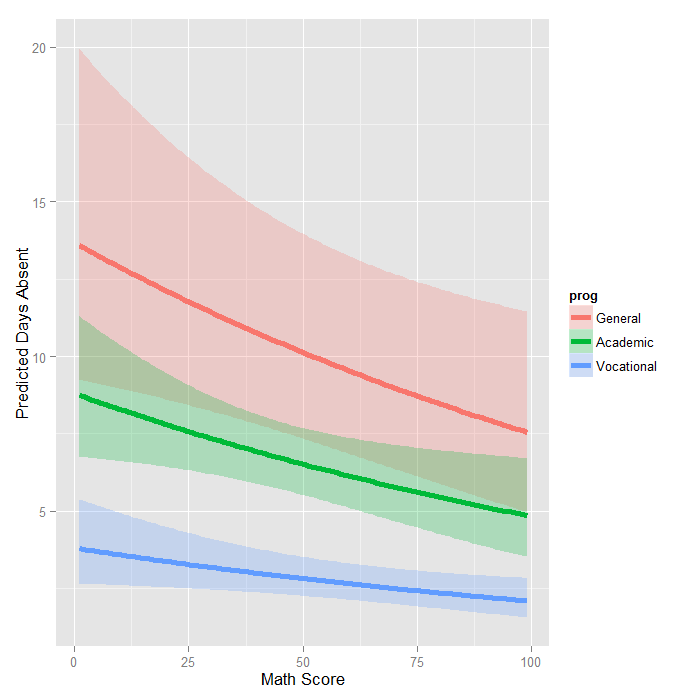
\includegraphics[width=0.7\linewidth]{negbin2}
		% \caption{}
		% \label{fig:negbin2}
\end{figure}
	
\end{frame}
\end{document}
